\chapter{Algoritmul Gorilla}
\label{chap:gorilla}

Acest capitol prezintă în detaliu algoritmul de compresie Gorilla, fundamentele sale matematice și schemele de codare utilizate. Algoritmul este compus din două tehnici complementare: \textbf{delta-of-delta encoding} pentru timestamp-uri și \textbf{XOR encoding} pentru valori în virgulă mobilă.

\section{Arhitectura generală}

\subsection{Structura datelor}

În Gorilla, datele sunt organizate în \textbf{blocuri} de durată fixă (implicit 2 ore). Fiecare bloc conține:

\begin{enumerate}
    \item Un \textbf{header} cu timestamp-ul de start al blocului (aliniat la granița de 2 ore);
    \item O secvență de perechi \textit{(timestamp, valoare)} comprimate;
    \item Metadate despre numărul de puncte din bloc.
\end{enumerate}

Alegerea blocurilor de 2 ore reprezintă un compromis între rata de compresie (blocuri mai mari = compresie mai bună) și granularitatea accesului (blocuri mai mici = citire mai rapidă pentru intervale scurte).

\subsection{Fluxul de compresie}

Schema generală de compresie este ilustrată în Figura~\ref{fig:compression-overview}.

\begin{figure}[h]
\centering
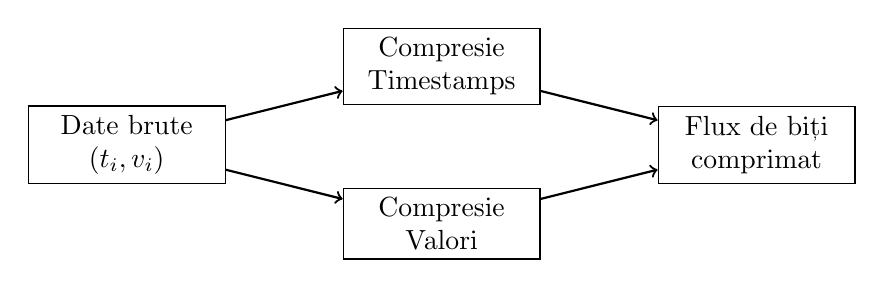
\begin{tikzpicture}[
    box/.style={draw, rectangle, minimum width=2.5cm, minimum height=0.8cm, align=center},
    arrow/.style={->, thick}
]
    % Input stream
    \node[box] (input) at (0,0) {Date brute\\$(t_i, v_i)$};

    % Timestamp compression
    \node[box] (ts) at (4,1) {Compresie\\Timestamps};

    % Value compression
    \node[box] (val) at (4,-1) {Compresie\\Valori};

    % Interleaved output
    \node[box] (output) at (8,0) {Flux de biți\\comprimat};

    % Arrows
    \draw[arrow] (input) -- (ts);
    \draw[arrow] (input) -- (val);
    \draw[arrow] (ts) -- (output);
    \draw[arrow] (val) -- (output);

\end{tikzpicture}
\caption{Fluxul general de compresie în Gorilla}
\label{fig:compression-overview}
\end{figure}

\section{Compresia Timestamp-urilor: Delta-of-Delta}
\label{sec:dod}

\subsection{Observația cheie}

Timestamp-urile în sistemele de monitorizare sunt de obicei \textbf{cvasi-periodice}. Dacă un sistem colectează date la fiecare 60 de secunde, timestamp-urile consecutive vor fi:
\begin{equation}
    t_0, t_0 + 60, t_0 + 120, t_0 + 180, \ldots
\end{equation}

Chiar dacă există mici variații (de exemplu, $t_0 + 61$ în loc de $t_0 + 60$), diferența $\delta_i = t_i - t_{i-1}$ rămâne aproape constantă.

\subsection{Delta encoding simplu}

Prima idee ar fi să stocăm diferențele (delta-urile) dintre timestamp-ul curent și cel anterior în loc de valoarea timstamp-ului curent:
\begin{equation}
    \delta_i = t_i - t_{i-1}
\end{equation}

Pentru timestamp-urile de mai sus: $\delta_1 = 60, \delta_2 = 60, \delta_3 = 60, \ldots$

Astfel reducem valorile de stocat de la 64 de biți (timestamp absolut) la câțiva biți (delta mic). Dar putem obține o stocare a datelor și mai eficientă!

\subsection{Delta-of-delta encoding}

Gorilla utilizează \textbf{delta-of-delta} (diferența diferențelor):
\begin{equation}
    D_i = \delta_i - \delta_{i-1} = (t_i - t_{i-1}) - (t_{i-1} - t_{i-2})
\end{equation}

Pentru timestamp-uri perfect periodice, $D_i = 0$ pentru toate $i > 1$. Aceasta este observația crucială: dacă timestamp-urile sunt regulate, \textbf{delta-of-delta este zero}.

\begin{example}
Să considerăm timestamp-urile: $1000, 1060, 1120, 1185, 1245$.

\begin{center}
\begin{tabular}{ccccc}
\toprule
$i$ & $t_i$ & $\delta_i = t_i - t_{i-1}$ & $D_i = \delta_i - \delta_{i-1}$ \\
\midrule
0 & 1000 & --- & --- \\
1 & 1060 & 60 & --- \\
2 & 1120 & 60 & 0 \\
3 & 1185 & 65 & +5 \\
4 & 1245 & 60 & -5 \\
\bottomrule
\end{tabular}
\end{center}

Observăm că $D_2 = 0$ (periodicitate perfectă), iar $D_3$ și $D_4$ sunt valori mici ($\pm 5$) care pot fi stocate eficient.
\end{example}

\subsection{Schema de codare variabilă}

Gorilla utilizează o schemă de codare cu lungime variabilă pentru valorile delta-of-delta, optimizată pentru distribuția observată în date reale:

\begin{table}[h]
\centering
\begin{tabular}{@{}lllc@{}}
\toprule
\textbf{Condiție} & \textbf{Prefix} & \textbf{Valoare} & \textbf{Total biți} \\
\midrule
$D = 0$ & \texttt{0} & --- & 1 \\
$D \in [-64, 63]$ & \texttt{10} & 7 biți signed & 9 \\
$D \in [-256, 255]$ & \texttt{110} & 9 biți signed & 12 \\
$D \in [-2048, 2047]$ & \texttt{1110} & 12 biți signed & 16 \\
Altfel & \texttt{1111} & 32 biți signed & 36 \\
\bottomrule
\end{tabular}
\caption{Schema de codare pentru delta-of-delta}
\label{tab:dod-encoding}
\end{table}

\subsection{Reprezentarea în complement față de 2}

Valorile delta-of-delta pot fi negative, deci trebuie reprezentate ca numere cu semn. Gorilla utilizează reprezentarea în \textbf{two's complement}.

Pentru un număr $x$ reprezentat pe $n$ biți:
\begin{itemize}
    \item Dacă $x \geq 0$: reprezentarea este $x$ în binar;
    \item Dacă $x < 0$: reprezentarea este $2^n + x$.
\end{itemize}

Intervalul reprezentabil pe $n$ biți este $[-2^{n-1}, 2^{n-1} - 1]$.

\begin{example}
Pentru $n = 7$ biți (intervalul $[-64, 63]$):
\begin{itemize}
    \item $x = 5$: reprezentare = $0000101_2$
    \item $x = -5$: reprezentare = $2^7 + (-5) = 128 - 5 = 123 = 1111011_2$
\end{itemize}
\end{example}

\subsection{Algoritmul de codare}

Este prezentat în cadrul \textbf{Algorithm 1}.

\begin{algorithm}[h]
\caption{Codare timestamp cu delta-of-delta}
\label{alg:ts-encode}
\begin{algorithmic}[1]
\Require Timestamp $t_n$, timestamp anterior $t_{n-1}$, delta anterior $\delta_{n-1}$
\Ensure Biți scriși în fluxul de ieșire

\State $\delta_n \gets t_n - t_{n-1}$
\State $D \gets \delta_n - \delta_{n-1}$

\If{$D = 0$}
    \State \textbf{write} \texttt{0} \Comment{1 bit}
\ElsIf{$-64 \leq D \leq 63$}
    \State \textbf{write} \texttt{10} \Comment{2 biți prefix}
    \State \textbf{write} $D$ pe 7 biți în complement față de 2
\ElsIf{$-256 \leq D \leq 255$}
    \State \textbf{write} \texttt{110} \Comment{3 biți prefix}
    \State \textbf{write} $D$ pe 9 biți în complement față de 2
\ElsIf{$-2048 \leq D \leq 2047$}
    \State \textbf{write} \texttt{1110} \Comment{4 biți prefix}
    \State \textbf{write} $D$ pe 12 biți în complement față de 2
\Else
    \State \textbf{write} \texttt{1111} \Comment{4 biți prefix}
    \State \textbf{write} $D$ pe 32 biți în complement față de 2
\EndIf

\State \Return $\delta_n$ \Comment{pentru următoarea iterație}
\end{algorithmic}
\end{algorithm}

\subsection{Algoritmul de decodare}

Decodarea citește biții de control pentru a determina lungimea valorii. Vezi \textbf{Algorithm 2}.

\begin{algorithm}[h]
\caption{Decodare timestamp}
\label{alg:ts-decode}
\begin{algorithmic}[1]
\Require Flux de biți, timestamp anterior $t_{n-1}$, delta anterior $\delta_{n-1}$
\Ensure Timestamp decodat $t_n$

\State $b_1 \gets$ \textbf{read} 1 bit
\If{$b_1 = 0$}
    \State $D \gets 0$
\Else
    \State $b_2 \gets$ \textbf{read} 1 bit
    \If{$b_2 = 0$}
        \State $D \gets$ \textbf{read} 7 biți signed
    \Else
        \State $b_3 \gets$ \textbf{read} 1 bit
        \If{$b_3 = 0$}
            \State $D \gets$ \textbf{read} 9 biți signed
        \Else
            \State $b_4 \gets$ \textbf{read} 1 bit
            \If{$b_4 = 0$}
                \State $D \gets$ \textbf{read} 12 biți signed
            \Else
                \State $D \gets$ \textbf{read} 32 biți signed
            \EndIf
        \EndIf
    \EndIf
\EndIf

\State $\delta_n \gets \delta_{n-1} + D$
\State $t_n \gets t_{n-1} + \delta_n$
\State \Return $t_n$
\end{algorithmic}
\end{algorithm}

\subsection{Eficiența compresiei timestamp-urilor}

În datele reale de la Facebook, distribuția valorilor delta-of-delta este puternic concentrată în jurul lui zero:

\begin{itemize}
    \item \textbf{96.39\%} dintre timestamp-uri au $D = 0$ (comprimate la 1 bit);
    \item \textbf{3.35\%} au $D \in [-64, 63]$ (9 biți);
    \item \textbf{0.19\%} au $D \in [-256, 255]$ (12 biți);
    \item Restul utilizează 16 sau 36 de biți.
\end{itemize}

Media ponderată rezultă în aproximativ \textbf{1.5 biți per timestamp}, comparativ cu 64 de biți fără compresie.

\section{Compresia Valorilor: XOR Encoding}
\label{sec:xor}

\subsection{Provocarea compresiei floating-point}

Numerele în virgulă mobilă (floating-point) sunt reprezentate conform standardului IEEE 754. Un număr \textit{double} (64 biți) are structura:

\begin{figure}[h]
\centering
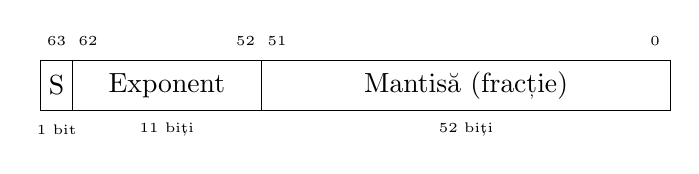
\begin{tikzpicture}[scale=0.8]
    % Sign bit
    \draw (0,0) rectangle (0.5,0.8);
    \node at (0.25,0.4) {S};
    \node at (0.25,-0.3) {\tiny 1 bit};

    % Exponent
    \draw (0.5,0) rectangle (3.5,0.8);
    \node at (2,0.4) {Exponent};
    \node at (2,-0.3) {\tiny 11 biți};

    % Mantissa
    \draw (3.5,0) rectangle (10,0.8);
    \node at (6.75,0.4) {Mantisă (fracție)};
    \node at (6.75,-0.3) {\tiny 52 biți};

    % Bit positions
    \node at (0.25,1.1) {\tiny 63};
    \node at (0.75,1.1) {\tiny 62};
    \node at (3.25,1.1) {\tiny 52};
    \node at (3.75,1.1) {\tiny 51};
    \node at (9.75,1.1) {\tiny 0};
\end{tikzpicture}
\caption{Structura IEEE 754 double-precision (64 biți)}
\label{fig:ieee754}
\end{figure}

Valoarea reprezentată este:
\begin{equation}
    v = (-1)^S \times 2^{E-1023} \times (1 + M/2^{52})
\end{equation}
unde $S$ este bitul de semn, $E$ este exponentul (11 biți), și $M$ este mantisa (52 biți).

\textbf{Problema}: Chiar și pentru valori foarte apropiate, reprezentările binare pot diferi semnificativ la nivelul mantisei. Delta encoding simplu nu funcționează eficient.

\subsection{Observația cheie: XOR pentru valori similare}

Gorilla exploatează o proprietate importantă: dacă două valori floating-point sunt \textit{apropiate numeric}, reprezentările lor binare tind să aibă mulți biți identici, în special în exponent și în biții superiori ai mantisei.

Operația \textbf{XOR} (exclusive OR) între două reprezentări binare produce:
\begin{itemize}
    \item \texttt{0} pentru biții identici;
    \item \texttt{1} pentru biții diferiți.
\end{itemize}

Pentru valori apropiate, XOR-ul va avea mulți \texttt{0} consecutivi la început (\textit{leading zeros}) și la sfârșit (\textit{trailing zeros}).

\begin{example}
Fie $v_1 = 24.0$ și $v_2 = 25.0$:
\begin{align*}
    v_1 &= \texttt{0x4038000000000000} \\
    v_2 &= \texttt{0x4039000000000000} \\
    v_1 \oplus v_2 &= \texttt{0x0001000000000000}
\end{align*}

XOR-ul are 15 leading zeros și 48 trailing zeros, lăsând doar 1 bit semnificativ!
\end{example}

\subsection{Schema de codare XOR}

Gorilla utilizează următoarea schemă pentru codarea valorilor:

\subsubsection{Prima valoare}
Prima valoare din bloc se stochează integral pe 64 de biți (necomprimată).

\subsubsection{Valori ulterioare}
Pentru fiecare valoare $v_n$ după prima:

\begin{enumerate}
    \item Calculăm $X = v_n \oplus v_{n-1}$ (XOR cu valoarea anterioară);

    \item \textbf{Dacă $X = 0$} (valori identice):
    \begin{itemize}
        \item Scriem un singur bit \texttt{0};
    \end{itemize}

    \item \textbf{Dacă $X \neq 0$}:
    \begin{itemize}
        \item Scriem bitul de control \texttt{1};
        \item Calculăm \textit{leading zeros} ($L$) și \textit{trailing zeros} ($T$);
        \item Numărul de biți semnificativi este: $M = 64 - L - T$;
    \end{itemize}

    \item \textbf{Dacă putem refolosi fereastra anterioară} ($L \geq L_{prev}$ și $T \geq T_{prev}$):
    \begin{itemize}
        \item Scriem bitul de control \texttt{0};
        \item Scriem doar biții semnificativi ($M_{prev}$ biți);
    \end{itemize}

    \item \textbf{Altfel} (definim o fereastră nouă):
    \begin{itemize}
        \item Scriem bitul de control \texttt{1};
        \item Scriem $L$ pe 5 biți (permite valori 0-31);
        \item Scriem $M - 1$ pe 6 biți (permite valori 1-64 codate ca 0-63);
        \item Scriem cei $M$ biți semnificativi din XOR.
    \end{itemize}
\end{enumerate}

\begin{table}[h]
\centering
\begin{tabular}{@{}lll@{}}
\toprule
\textbf{Caz} & \textbf{Format} & \textbf{Biți} \\
\midrule
XOR = 0 & \texttt{0} & 1 \\
Refolosim fereastra & \texttt{10} + meaningful bits & 2 + $M_{prev}$ \\
Fereastră nouă & \texttt{11} + 5 biți + 6 biți + meaningful bits & 13 + $M$ \\
\bottomrule
\end{tabular}
\caption{Schema de codare XOR pentru valori}
\label{tab:xor-encoding}
\end{table}

\subsection{Calculul leading și trailing zeros}

Fie $X$ rezultatul XOR reprezentat pe 64 de biți. Definim:

\begin{equation}
    L = \max\{i : \text{biții } 63, 62, \ldots, 64-i \text{ sunt toți } 0\}
\end{equation}

\begin{equation}
    T = \max\{j : \text{biții } 0, 1, \ldots, j-1 \text{ sunt toți } 0\}
\end{equation}

\begin{equation}
    M = 64 - L - T \quad \text{(biții semnificativi)}
\end{equation}

\begin{example}
Pentru $X = \texttt{0x0001000000000000}$:
\begin{itemize}
    \item Reprezentare binară: \texttt{0000...0001 0000...0000} (15 zeros, apoi 1, apoi 48 zeros)
    \item $L = 15$ (leading zeros)
    \item $T = 48$ (trailing zeros)
    \item $M = 64 - 15 - 48 = 1$ (un singur bit semnificativ)
\end{itemize}
\end{example}

\subsection{Algoritmul de codare pentru valori}

\begin{algorithm}[h]
\caption{Codare valoare cu XOR}
\label{alg:val-encode}
\begin{algorithmic}[1]
\Require Valoare $v_n$, valoare anterioară $v_{n-1}$ (ca biți), $L_{prev}$, $T_{prev}$
\Ensure Biți scriși în fluxul de ieșire

\State $X \gets v_n \oplus v_{n-1}$ \Comment{XOR între reprezentări pe 64 biți}

\If{$X = 0$}
    \State \textbf{write} \texttt{0} \Comment{1 bit --- valori identice}
\Else
    \State \textbf{write} \texttt{1} \Comment{bit de control}
    \State $L \gets$ \Call{CountLeadingZeros}{$X$}
    \State $T \gets$ \Call{CountTrailingZeros}{$X$}
    \State $M \gets 64 - L - T$

    \If{$L \geq L_{prev}$ \textbf{and} $T \geq T_{prev}$}
        \State \textbf{write} \texttt{0} \Comment{refolosim fereastra}
        \State $M_{use} \gets 64 - L_{prev} - T_{prev}$
        \State \textbf{write} biții semnificativi din $X$ ($M_{use}$ biți)
    \Else
        \State \textbf{write} \texttt{1} \Comment{fereastră nouă}
        \State \textbf{write} $\min(L, 31)$ pe 5 biți
        \State \textbf{write} $(M - 1)$ pe 6 biți
        \State \textbf{write} biții semnificativi din $X$ ($M$ biți)
        \State $L_{prev} \gets L$; $T_{prev} \gets T$
    \EndIf
\EndIf
\end{algorithmic}
\end{algorithm}

\subsection{Eficiența compresiei valorilor}

În datele Facebook:
\begin{itemize}
    \item \textbf{59.06\%} dintre valori sunt identice cu precedenta (1 bit);
    \item \textbf{28.30\%} refolosesc fereastra anterioară (~27 biți în medie);
    \item \textbf{12.64\%} necesită fereastră nouă (~40 biți în medie).
\end{itemize}

Media rezultă în aproximativ \textbf{12-15 biți per valoare}, comparativ cu 64 de biți fără compresie.

\section{Compresia combinată}

Rata totală de compresie pentru o pereche (timestamp, valoare) este:
\begin{equation}
    R = \frac{128 \text{ biți}}{b_{ts} + b_{val}}
\end{equation}
unde $b_{ts}$ și $b_{val}$ sunt biții necesari pentru timestamp și valoare.

În practică, Gorilla obține în medie \textbf{1.37 bytes per punct} (11 biți), comparativ cu 16 bytes necomprimat, reprezentând o rată de compresie de aproximativ \textbf{12x}.

\section{Analiza complexității}

\subsection{Complexitate temporală}

\textbf{Codare (per punct)}: $O(1)$
\begin{itemize}
    \item Calcul delta/XOR: $O(1)$
    \item Scriere biți: $O(k)$ unde $k$ este numărul de biți (constant, maxim 100)
\end{itemize}

\textbf{Decodare (per punct)}: $O(1)$
\begin{itemize}
    \item Citire biți de control: $O(1)$
    \item Reconstrucție valoare: $O(1)$
\end{itemize}

\subsection{Complexitate spațială}

\textbf{Stare per encoder}: $O(1)$
\begin{itemize}
    \item Timestamp anterior: 8 bytes
    \item Delta anterior: 8 bytes
    \item Valoare anterioară: 8 bytes
    \item Leading/trailing zeros anteriori: 2 bytes
\end{itemize}

\textbf{Buffer de ieșire}: $O(n)$ unde $n$ este numărul de puncte, dar cu factor constant mic ($\approx 1.37$ bytes/punct în loc de 16).

\section{Extindere pentru serii multivariate}

O serie \textbf{multivariată} conține mai multe valori per timestamp:
\begin{equation}
    (t_i, v_i^{(1)}, v_i^{(2)}, \ldots, v_i^{(k)})
\end{equation}

\subsection{Strategia de compresie}

Abordarea naivă ar fi să tratăm fiecare variabilă ca o serie separată, dar aceasta ar duplica timestamp-urile de $k$ ori.

Gorilla pentru serii multivariate utilizează:
\begin{enumerate}
    \item \textbf{Un singur stream de timestamp-uri} (delta-of-delta);
    \item \textbf{Câte un stream separat pentru fiecare variabilă} (XOR encoding).
\end{enumerate}

Toate stream-urile scriu în același buffer de biți, dar fiecare variabilă își menține propriul context XOR (valoare anterioară, leading/trailing zeros).